\documentclass{beamer}

\usetheme{Copenhagen}
\usecolortheme{lily}
\usepackage[T1]{fontenc}
\usepackage[ansinew]{inputenc}
\usepackage[USenglish]{babel}
\usepackage{amsmath}
\usepackage{mathtools}
\usepackage{stmaryrd}
\usepackage{graphicx}
\usepackage{lmodern}


\usepackage[round, authoryear]{natbib}

\newcommand\Wider[2][3em]{%
\makebox[\linewidth][c]{%
  \begin{minipage}{\dimexpr\textwidth+#1\relax}
  \raggedright#2
  \end{minipage}%
  }%
}


\DeclareMathOperator*{\plim}{plim}

\setbeamertemplate{footline}[frame number]

\begin{document}



\title{Classifying Refugee News Reports}
\subtitle{Data Warehousing and Computing Lab}

\author{Euan Dowers, Robert Lange, Nandan Rao \\ Supervisors: G. Bartolozzi and C. Brownlees \\ Barcelona Graduate School of Economics}
\date{\today}


%------------------------------------------------------------------------------%

\begin{frame}
\titlepage
\end{frame}

%------------------------------------------------------------------------------%
\section*{Overview}

\begin{frame}{Outline}
\nocite{*}
\begin{enumerate}
	\item \textbf{Aim and Motivation}\\
		\small{Working with IOM and Refugee News Flood}
	\item \textbf{Database Management}\\
	    \small{UI, Architecture, Persistance}\\
	\item \textbf{Text Processing}\\
	    \small{String Cleaning, Vectorization and tf-idf Representations}
	\item \textbf{Modelling the Data} \\
	    \small{Clustering and Cross-Validated Classifiers}  
\end{enumerate}	

\end{frame}


%------------------------------------------------------------------------------%
\begin{frame}{Motivation - Missing Migrant Project (MMP)}

%\begin{itemize}

%\item Refugee crisis, war in Syria $\Rightarrow$ increase in news reports and rumors regarding missing migrants.
%\item Awareness and efficient allocation of resources 
%\item International Organisation for Migration (IOM)

%	\begin{itemize}
%	\item[$\to$] Missing Migrant Project
%	\end{itemize}

%\end{itemize}

\begin{figure}[H]
\centering
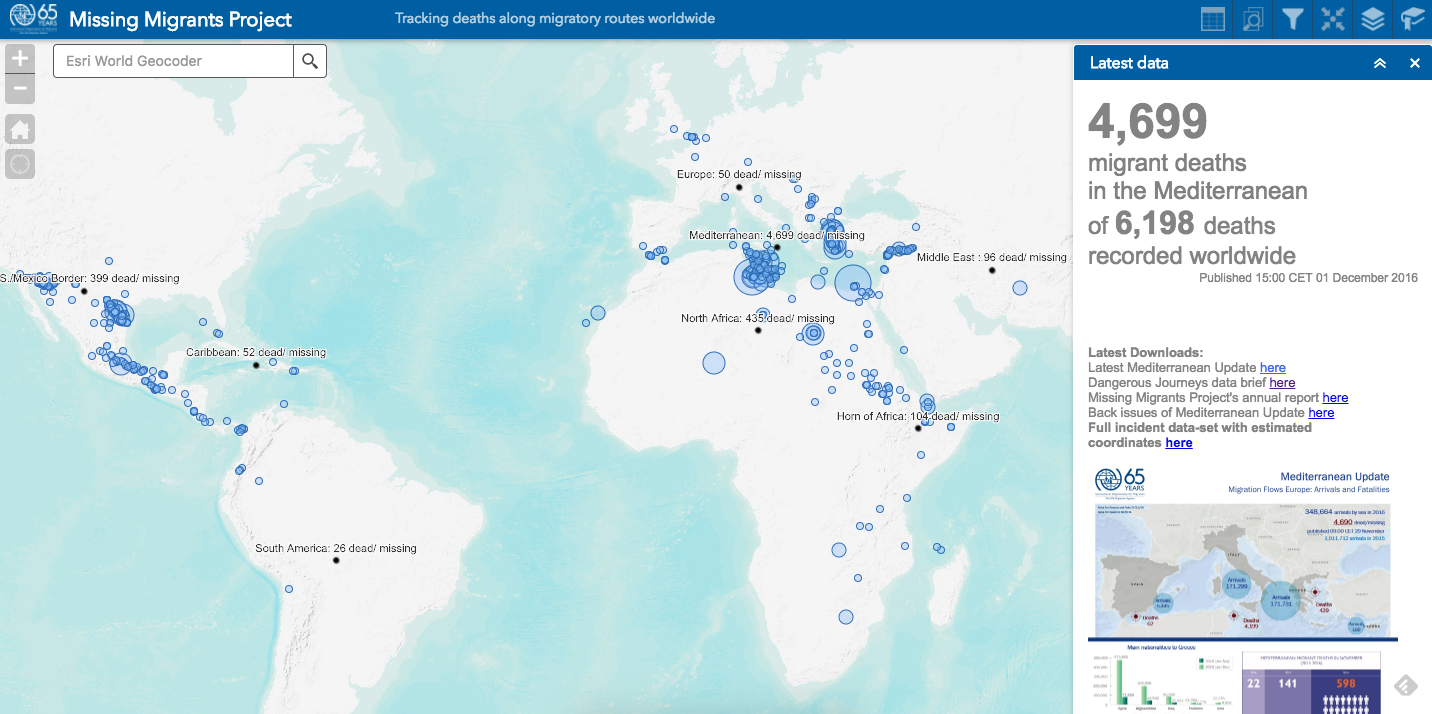
\includegraphics[scale=0.225]{MMP.png}
\label{heat}
\end{figure}

\href{https://missingmigrants.iom.int/}{\beamergotobutton{Link}}

\end{frame}

%------------------------------------------------------------------------------%
\section{Database Management}
%------------------------------------------------------------------------------%

\begin{frame}{Data Types, Challenges and a Solution}
\begin{itemize}
\item Data Sources:

	\begin{itemize}
		\item[$\rightarrow$] Google Alert News Feeds
		\item[$\rightarrow$] Twitter Feeds
		\item[$\rightarrow$] Missing Migrant Project (MMP) data
	\end{itemize}

\item Data Management Challenges:

	\begin{itemize}
		\item[$\rightarrow$] One schema is not enough (different data types)
		\item[$\rightarrow$] Online data integration
		\item[$\rightarrow$] Pulling from different news feeds
	\end{itemize}
	
\item Data Management Solution: MongoDB	

\end{itemize}
\end{frame}


%------------------------------------------------------------------------------%

\begin{frame}{Architecture and Persistance}
\begin{itemize}
\item MongoDB has several advantages:
\end{itemize}
\end{frame}

%------------------------------------------------------------------------------%
%------------------------------------------------------------------------------%
\section{Text Processing}

%------------------------------------------------------------------------------%

\begin{frame}{Cleaning the strings}

\begin{itemize}
\item Original text string - Label: Rejected
\end{itemize}

\Wider{
\begin{figure}[H]
\centering
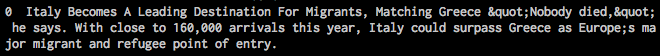
\includegraphics[scale=0.5]{Text_Processing/1.png}
\label{heat}
\end{figure}
}

\begin{itemize}
\item Splitting text into tokens
\end{itemize}

\Wider{
\begin{figure}[H]
\centering

\includegraphics[scale=0.5]{Text_Processing/2.png}
\label{heat}
\end{figure}
}

\begin{itemize}
\item Removing stopwords and lemma transformation
\end{itemize}

\Wider{
\begin{figure}[H]
\centering
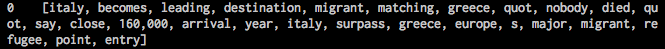
\includegraphics[scale=0.5]{Text_Processing/3.png}
\label{heat}
\end{figure}
}

\end{frame}
%------------------------------------------------------------------------------%

\begin{frame}{Constructing a Vectorized Representation}
\begin{itemize}
\item Count Vectorization
\item tf-idf: re-weighting by proportion of times a word appears in the document vs. corpus
\item Deciding on dimensionality: bi-grams, tri-grams, etc.
	\begin{itemize}
		\item[$\to$] Which representations do really matter?
	\end{itemize}
 
\end{itemize}
\end{frame}

%------------------------------------------------------------------------------%
%------------------------------------------------------------------------------%
\section{Modelling the Data}
%------------------------------------------------------------------------------%
%\begin{frame}{The Problem}
%\begin{itemize}

%\item Easy/accelerated classification of relevant and irrelevant news
%\item Problems:
%	\begin{enumerate}
%		\item Redundancy: Many observations cover the same events
%		\item Sensitivity: Hard classification problem
%	\end{enumerate}

%\item Solutions: 
%	\begin{enumerate}
%		\item Hierarchical clustering using DBSCAN
%		\item Ensemble Methods: Random Forest
%	\end{enumerate}

%\end{itemize}
%\end{frame}

%------------------------------------------------------------------------------%
\begin{frame}{Building a First Classification Model}

\begin{itemize}
	\item Many potential classifiers available: Logistic Regression, Naive Bayes, SVM,
Decision Tree, Random Forest and NNs
	\item Idea: Start with MVP (minimal viable product) to grasp the problem $\to$ Generative Model: Naive Bayes
	
	$$ p(t_j|x_i) = p(x_i|t_j) p(t_j) p(x_i)$$
	
	\begin{itemize}
		\item Assumption: Treat observations as iid $\to$ likelihood factorizes
	\end{itemize}
	
	
	$$p(x|t) = \prod_{k=1}^d p(x_k|t_j)$$

\end{itemize}
\end{frame}

%------------------------------------------------------------------------------%
\begin{frame}{Model Evaluation}

\begin{figure}
\centering

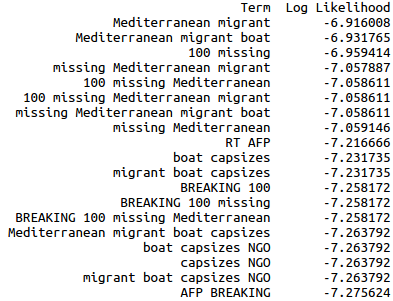
\includegraphics[scale=0.5]{nbterms.png}
\label{naivebayes}


\end{figure}

\end{frame}

%------------------------------------------------------------------------------%
\begin{frame}{Model Evaluation}

\begin{figure}
\centering

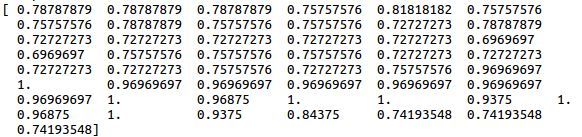
\includegraphics[scale=0.5]{naivebayesscores.png}
\label{naivebayes}

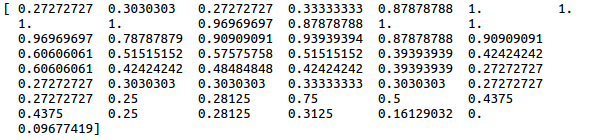
\includegraphics[scale=0.5]{naivebayesnoprior.png}
\label{naivebayes}


\end{figure}

\end{frame}

%------------------------------------------------------------------------------%
\begin{frame}{Adding Complexity: Random Forests}

\begin{figure}
\centering

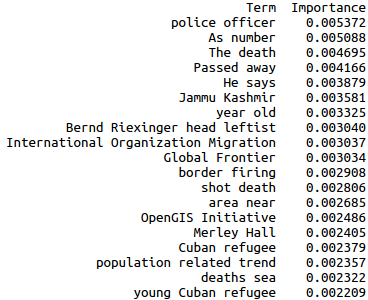
\includegraphics[scale=0.5]{randomforestvis.png}
\label{randomforest}

\end{figure}

\end{frame}

%------------------------------------------------------------------------------%
\begin{frame}{Adding Complexity: Random Forests}

\begin{figure}
\centering

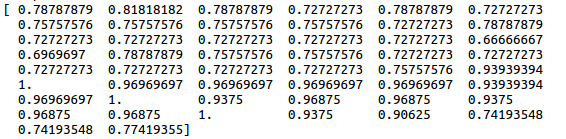
\includegraphics[scale=0.5]{randomforestscores.png}
\label{randomforest}

\end{figure}

\end{frame}

%------------------------------------------------------------------------------%

\begin{frame}{Automated Labelling Process and Lean UX}

\begin{figure}[H]
\centering
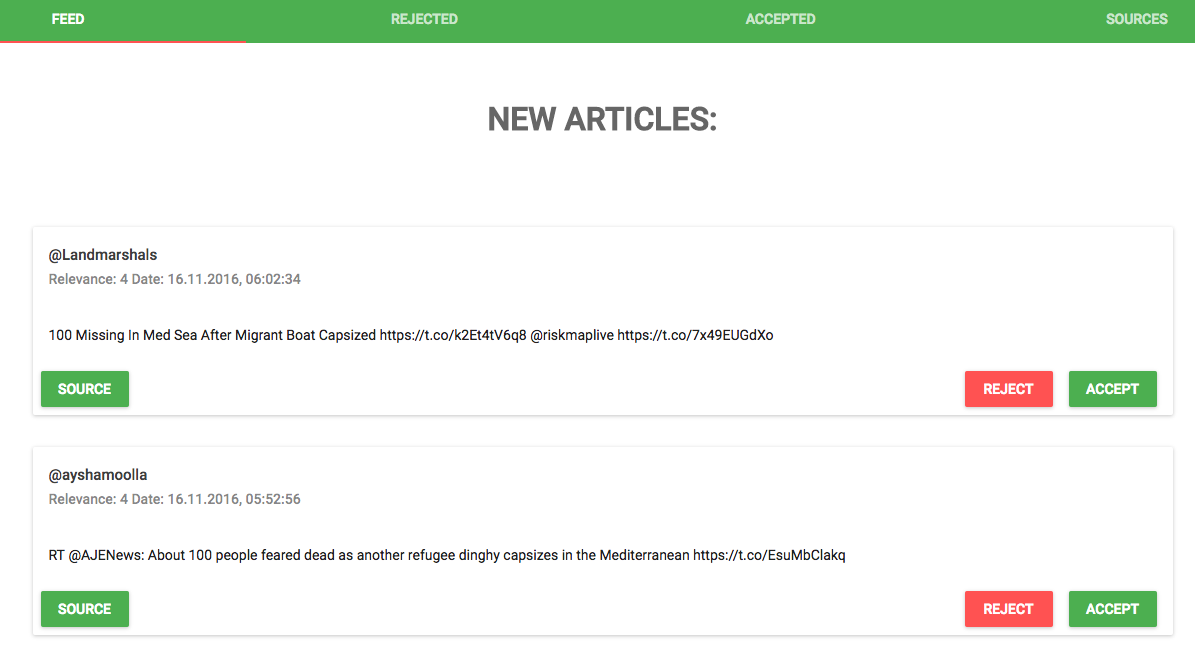
\includegraphics[scale=0.25]{UI.png}
\label{heat}
\end{figure}

\href{http://migrantnews-web.s3-website-eu-west-1.amazonaws.com/}{\beamergotobutton{Link}}

\end{frame}

%------------------------------------------------------------------------------%
\begin{frame}{Clustering using DBSCAN - Density-based spatial clustering of applications with noise}

\begin{itemize}
    \item Density based clustering algorithm that takes as parameters $\epsilon$ and $n$ minimum points in a cluster. 
    \item DBSCAN allows points to be marked as noise - not in any cluster
    \item Do not need to specify number of clusters before running DBSCAN
    \item Intention is to cluster similar stories/tweets using vectorized presentation. 
\end{itemize}

\end{frame}

%------------------------------------------------------------------------------%
\begin{frame}{Problems and Improving Classification}

\begin{itemize}
	\item Sensitivity to specific "small" words: e.g. not
\end{itemize}

\begin{itemize}
	\item Hyperparameter choices: 5-fold cross-validation and parameter grid search
	\item Adding non-parametric complexity: Random Forest
\end{itemize}

\end{frame}


%------------------------------------------------------------------------------%
\begin{frame}{Conclusion}

\begin{itemize}
\item Open research/work:
\begin{enumerate}
\item Better understanding of the decision boundary problem
\end{enumerate}
\item \Large{\textit{Any Questions?}}
\item \Large{\textit{Thank you for your attention!}}
\end{itemize}


\end{frame}
%------------------------------------------------------------------------------%

%\begin{frame}[allowframebreaks]{References}
 %   \begin{scriptsize}
  %   %\nocite{*}  // commented out!!!!!!!!
   %  \setbeamertemplate{bibliography item}[text]
    % \bibliographystyle{authordate1}
     %\bibliography{dynamicpanels}
    %\end{scriptsize}
    %\end{frame}

%------------------------------------------------------------------------------%

\end{document} 